\documentclass[hidelinks]{report}
\usepackage{graphicx} % Required for inserting images
\usepackage{amsmath}
\usepackage{siunitx}
\usepackage{placeins}
\usepackage{float}
\usepackage{hyperref}
\usepackage{cite}
\usepackage[utf8]{inputenc}
\usepackage[T1]{fontenc}
\usepackage{xcolor,graphicx}
\setcounter{secnumdepth}{0}
\usepackage{titlesec}
\usepackage[left=1.5in,top=1in,bottom=1in,right=1in]{geometry}
\usepackage{rotating}
\usepackage{subcaption}
\usepackage{lipsum}
\usepackage{fancyhdr}
\usepackage{mathptmx}
\usepackage{listings}
\usepackage{booktabs}
\usepackage{caption}
\usepackage{subcaption}
\usepackage{adjustbox}
\usepackage{enumitem}
\usepackage{setspace}
\usepackage{multirow}
\usepackage{tikz}
\setcounter{tocdepth}{4}
\usepackage{amsfonts}
\usepackage{pdflscape}
\usepackage{booktabs} 
\usepackage{array} 

\newcommand{\mynote}[2]{\fbox{\bfseries\sffamily\scriptsize{#1}} {\small\textsf{\emph{#2}}}}

\newcommand{\hieplnc}[1]{\textcolor{red}{\mynote{hieplnc}{#1}}}

\newcommand{\sontg}[1]{\textcolor{blue}{\mynote{sontg}{#1}}}

\definecolor{blue}{RGB}{31,56,100}

\usepackage{lipsum}% http://ctan.org/pkg/lipsum
\makeatletter
\def\@makechapterhead#1{%
  {%
    \parindent \z@ \normalfont % No specific alignment for full justification
    
    \ifnum \c@secnumdepth >\m@ne
        \LARGE\bfseries \thechapter.\ % Changed to \Large (smaller than \LARGE)
    \fi
    \interlinepenalty\@M
    \LARGE\bfseries % Reduced from \LARGE to \Large
    #1\par\nobreak% <------------------ Chapter title
    \vskip 40\p@% <------------------ Space between chapter title and first paragraph
  }%
}

\def\@makeschapterhead#1{%
  {%
    \parindent \z@ \normalfont % No specific alignment for full justification
    \interlinepenalty\@M
    \LARGE\bfseries % Reduced from \LARGE to \Large
    #1\par\nobreak% <------------------ Chapter title
    \vskip 40\p@% <------------------ Space between chapter title and first paragraph
  }%
}
\makeatother

% Redefine the \thesection and \thesubsection representations
\renewcommand{\thesection}{\arabic{chapter}.\arabic{section}}
\renewcommand{\thesubsection}{\thesection.\arabic{subsection}}
\renewcommand{\thesubsubsection}{\thesubsection.\arabic{subsubsection}}

% Define a new counter for subsections
% \newcounter{subsecindex}[section]
% \renewcommand{\thesubsecindex}{\thesubsection%
%   \ifnum\value{subsecindex}>0
%     .\arabic{subsecindex}%
%   \fi
% }

% Redefine the \section command to include the index
% \let\oldsection\section
% \renewcommand{\section}[1]{%
%   \setcounter{subsecindex}{0} % Reset subsection counter for each section
%   \refstepcounter{section}%
%   \oldsection{\thesection\hspace{0.5em}#1}%
% }

% Redefine the \subsection command to include the index
% \let\oldsubsection\subsection
% \renewcommand{\subsection}[1]{%
%   \refstepcounter{subsection}%
%   \oldsubsection{\thesubsecindex\hspace{0.5em}#1}%
% }

% Redefine the \subsubsection command to include the index
% \let\oldsubsubsection\subsubsection
% \renewcommand{\subsubsection}[1]{%
%   \refstepcounter{subsubsection}%
%   \oldsubsubsection{\thesubsecindex\hspace{0.5em}#1}%
% }

\titleformat{\section}
  {\normalfont\LARGE\bfseries} % Adjust \Large to any size you prefer
  {\thesection}{3em}{}
\titleformat{\subsection}
  {\normalfont\Large\bfseries} % Adjust \Large to any size you prefer
  {\thesubsection}{3em}{}
\titleformat{\subsubsection}
  {\normalfont\Large\bfseries} % Adjust \Large to any size you prefer
  {\thesubsubsection}{3em}{}

\begin{document}
\pagenumbering{gobble}

\pdfbookmark[0]{Main Title}{maintitle}
\begin{titlepage}
    \begin{tikzpicture}[remember picture,overlay,inner sep=0,outer sep=0]
        \draw[black!70!black,line width=1.5pt]
            ([xshift=-0.65in,yshift=-1cm]current page.north east) coordinate (A) -- % Adjusted x-shift and y-shift
            ([xshift=0.65in,yshift=-1cm]current page.north west) coordinate (B) -- % Adjusted x-shift and y-shift
            ([xshift=0.65in,yshift=1cm]current page.south west) coordinate (C) -- % Adjusted x-shift and y-shift
            ([xshift=-0.65in,yshift=1cm]current page.south east) -- % Adjusted x-shift
            cycle;
    \end{tikzpicture}

    \begin{center}
        \huge \uppercase{University of Science and Technology of Hanoi} \\ [1.5 cm]
    
        
\includegraphics[width=0.9\linewidth]{image/usth.png} \\[1cm]

        {\huge \bfseries \uppercase{MASTER LABWORK}} \\[1cm]

        {\large \bfseries Nguyen Viet Tung} \\ [0.5cm]
        {\large \bfseries 2440049} \\ [0.7cm]
        {\huge \bfseries \uppercase{Deep Learning}} \\[1cm]
        
        % Title
        \rule{\linewidth}{0.3mm} \\[0.4cm]
        { \Huge \bfseries\color{blue} Labwork 1: Gradient Descent \\[0.4cm] }
        \rule{\linewidth}{0.3mm} \\[0.7cm]
        
        \large Academic Year: 2024-2026
    \end{center}

\end{titlepage}

\newpage
\pagenumbering{roman}
\tableofcontents

\newpage
\listoffigures

\thispagestyle{empty}
\newpage
\pagenumbering{arabic}

\begin{abstract}
    Implement (from scratch!) gradient descend to find minimum value of a given function f(x) and its first order derivative f\_()
        \begin{itemize}
            \item Print the intermediate iterative steps, similar to the previous table (time, x, f(x))
            \item Try experimenting with the previous example f(x) = $x^2$   
        \end{itemize}

\end{abstract}


\chapter{How you implement the algorithm.}

\section{Mathematical Background}
Gradient descent is an optimization algorithm used to minimize a function by iteratively moving in the direction of steepest descent, which is defined by the negative of the gradient. For a function $f(x)$, the update rule is:

\begin{equation}
x_{t+1} = x_t - \alpha \nabla f(x_t)
\end{equation}

where $\alpha$ is the learning rate and $\nabla f(x_t)$ is the gradient of the function at point $x_t$.

\section{Implementation Details}
\noindent For this exercise, we implement the gradient descent to find the minimum value of $f(x) = x^2$. The derivative of this function is $f'(x) = 2x$. The algorithm is implemented from scratch in Python, with the following components:

\subsection{Function and Derivative Definition}
\noindent First, we define the function to minimize and its derivative:

\begin{verbatim}
def test_function(x):
    return x**2

def df(x):
    return 2*x
\end{verbatim}

\subsection{Gradient Descent Algorithm}
\noindent The core algorithm is implemented as follows:

\begin{verbatim}
def gradient_descent(starting_point, learning_rate=0.1, num_iterations=20):
    x = starting_point
    iteration = 0
    history = []
    
    while iteration < num_iterations:
        gradient = df(x)
        history.append({'iteration': iteration, 'x': x, 'gradient': gradient})
        iteration += 1
        x = x - learning_rate * gradient
        
    result = pd.DataFrame(history)
    result['f(x)'] = test_function(result['x'])
    return result
\end{verbatim}

\noindent This implementation:
\begin{itemize}
    \item Takes a starting point, learning rate, and number of iterations as parameters
    \item Initializes $x$ with the starting point
    \item Iteratively computes the gradient at the current point
    \item Updates $x$ using the update rule: $x = x - \alpha \times \text{gradient}$
    \item Records the history of iterations including iteration number, $x$ value, and gradient
    \item Returns a pandas DataFrame with the history and $f(x)$ values
\end{itemize}

\section{Experimental Setup}
\noindent To analyze the effect of different learning rates on convergence, we test the algorithm with multiple learning rates:

\begin{verbatim}
starting_point = 5
learning_rate = [1, 0.1, 0.01, 0.001]
num_iterations = 50
\end{verbatim}

\noindent For each learning rate, we:
\begin{itemize}
    \item Run the gradient descent algorithm
    \item Store the results with the corresponding learning rate
    \item Visualize the convergence path using a 2×2 grid of plots
\end{itemize}

\section{Analysis of Results}
\noindent The visualization shows how different learning rates affect the convergence behavior:

\begin{figure}[H]
    \centering
    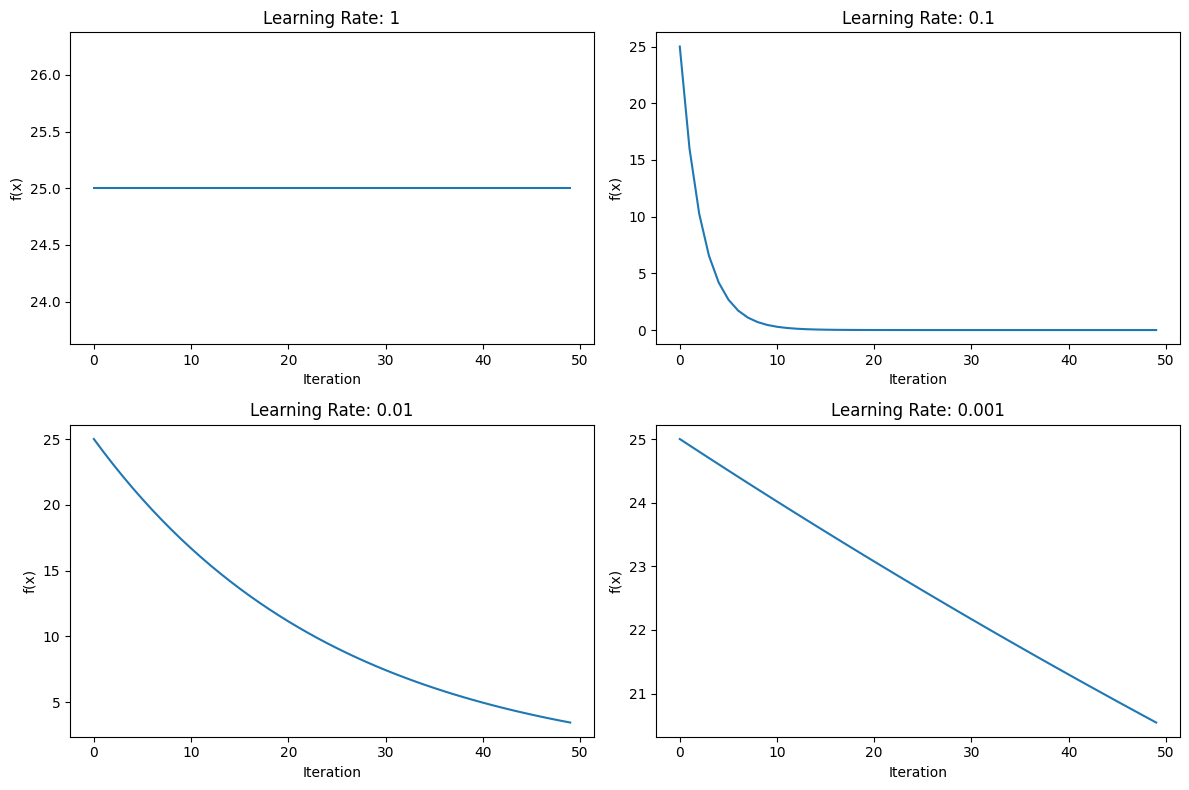
\includegraphics[width=1\linewidth]{image/learning-rate-comparision.png}
    \caption{Convergence behavior of gradient descent with different learning rates}
    \label{fig:enter-label}
\end{figure}

\begin{itemize}
    \item \textbf{Learning Rate 1.0}: The algorithm oscillates and fails to converge, demonstrating that too large a learning rate can cause the algorithm to overshoot the minimum.
    \item \textbf{Learning Rate 0.1}: Shows optimal convergence behavior, quickly reaching the minimum.
    \item \textbf{Learning Rate 0.01}: Converges more slowly but steadily.
    \item \textbf{Learning Rate 0.001}: Exhibits extremely slow convergence, demonstrating that too small a learning rate is inefficient.
\end{itemize}

\noindent This implementation demonstrates the critical importance of selecting an appropriate learning rate for gradient descent optimization.

    
\clearpage
\pagenumbering{gobble}

\end{document}